\chapter{Application}
\section{Architecture}
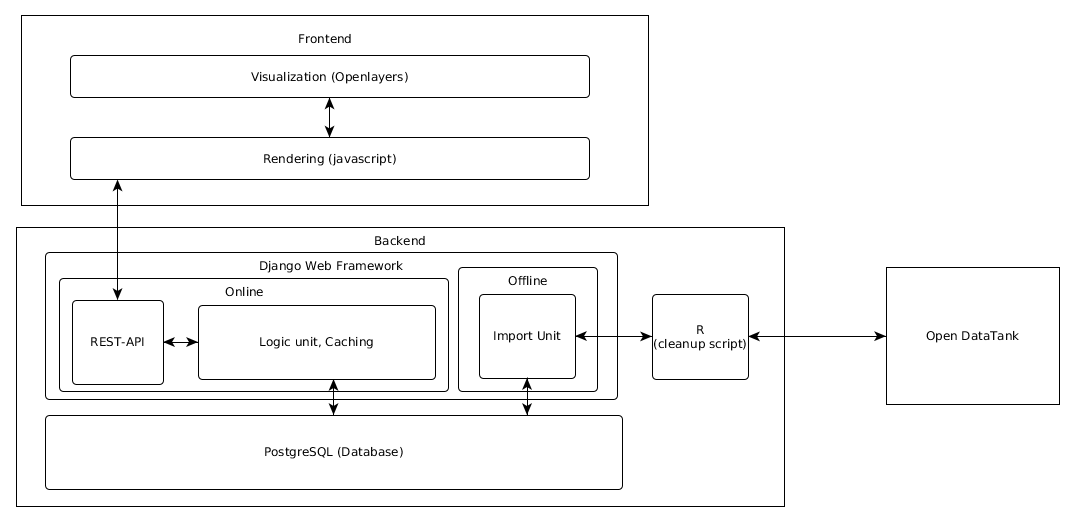
\includegraphics[width=16cm]{fig/Architecture}

\subsection{Frontend}
At the frontend side of our web application, we will have two main components, a rendering component and a visualization component. At the rendering block, the data requested via the API from the backend will be transformed into e.g. figures, dots, that can be displayed on the browser. When the transformation is finished, the visualization block will show the transformed data on the website itself.

\subsection{Backend}
We make use of 3 main components in the backend. First there is the RML unit which will be used to make a mapping between the data of the Open Datatank towards a Linked Data JSON format. The second component is the database, for which we will use MongoDB so we can create a semantical database. As last main component, we have the django web framework. The blocks in this framework consist of an online and offline section. In the online section we have the REST-API which will be used to open up our data to our website and also towards other applications because of the open data concept. Besides this REST-API there is also a logical unit where the caching of requests, data,... will happen. At the offline section of the Django Web Framework, we will provide an import unit to put the JSON-LD data into the database. This is an offline block since the data is provided as a data dump and only needs to imported once. Since it will make use of the mapping that Django provides between the database and Python objects, it is included in the Django block.

\section{Functional requirements}

\subsection{User interface}

On initial load of the webpage an empty map of Ghent is shown with one big number counting the sum of all books ever loaned. This map is divided in statistical sectors. The shape of these sectors is dynamic (online available) and will be retrieved every time the page is loaded. Under the map will be a slider showing the time span for the data published. Every sector can be selected, if none is, the data represented is for all of Ghent.  The numbers shown are the amount of books that fit the query. The query is defined by the optional arguments; sector, time span and properties of the books. An example; sector="A2", book: genre="horror". This query will give the amount of horror books loaned in sector A2 from the oldest (1996) to the youngest (2014) data (because time span is not specified). The book properties of the query are given in an input section above the map. Also shown on the map are distribution locations (libraries). A second layer of visualised data shows where books are loaned from. This relation between statistical sector and library can be visualised by a line. The user can zoom in and out on this map and it's visualised data by scrolling.

\section{Use case}

The library personel can use the web application in two ways, reactively and pro-actively. Respectively by searching on a specific book (title) or on a certain group of books (genre, target-age,...) and look for differences between current distribution (visualised per library) and preffered distribution (visualised per sector). If the demand of a certain book is skewed for a sector, the copies can be moved closer (closer library) to this sector. If the demand of a group correlates with a sector the personel can decide to anticipate the demand of similar books in this group and move the whole group.
